\section{IT Applications} 
\begin{frame}
	\frametitle{Certificate Course in Software Testing}
		\begin{columns}
		
		\column{0.45\textwidth}
		
		\begin{figure}
			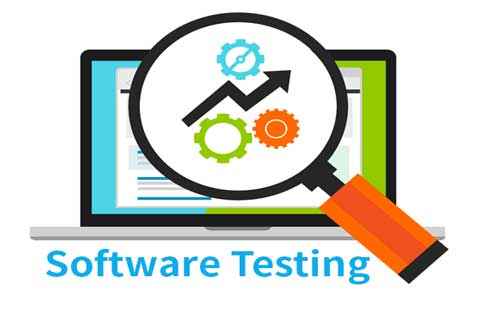
\includegraphics[width=200pt,height=150pt]{figures/course_st.jpg}
		\end{figure}
		
		\column{0.55\textwidth}
		
		\begin{block}{Description}
			
			\begin{enumerate}
				\item Software Development Life Cycle. 
				\item Software Testing – Manual.
				\item Software Testing – Automation.
			\end{enumerate}
			
		\end{block}
		
	\end{columns}
\end{frame}
\begin{frame}
	\frametitle{Certificate Course in Office Automation}
		\begin{columns}
		
		\column{0.45\textwidth}
		
		\begin{figure}
			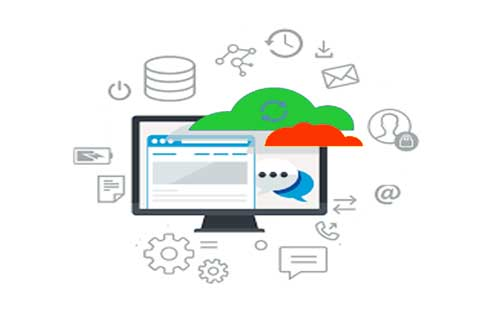
\includegraphics[width=200pt,height=150pt]{figures/course_oa.jpg}
		\end{figure}
		
		\column{0.55\textwidth}
		
		\begin{block}{Description}
			
			\begin{enumerate}
				\item Client Operating System (Windows 10, Ubuntu). 
				\item MS Office 2016
				\item Database Concepts
				\item Database Management using MS access
			\end{enumerate}
			
		\end{block}
		
	\end{columns}
\end{frame}
\begin{frame}
	\frametitle{Certificate Course in Information Technology}
		\begin{columns}
		
		\column{0.45\textwidth}
		
		\begin{figure}
			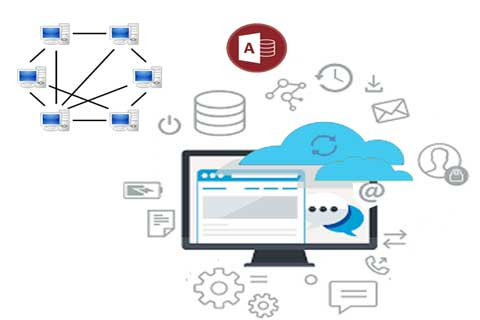
\includegraphics[width=200pt,height=150pt]{figures/course_it.jpg}
		\end{figure}
		
		\column{0.55\textwidth}
		
		\begin{block}{Description}
			
			\begin{enumerate}
				\item Office Automation Tools. 
				\item Computer Fundamentals.
				\item Communication using PC.
				\item Overview of Networking.
				\item Database Concepts and MS Access.
			\end{enumerate}
			
		\end{block}
		
	\end{columns}
\end{frame}